\newcommand{\ConstExercise}{4}
\newcommand{\ConstDeadline}{05.05.2023}

\documentclass[11pt,letterpaper]{article}
\textwidth 6.5in
\textheight 9.in
\oddsidemargin 0in
\headheight 0in

\usepackage[exp]{custom_0.1}

\begin{document}

%%%%% Document %%%%%

\begin{enumerate}
    \item \textbf{Wärmebad, Gas zusammendrücken}
        \begin{enumerate}
            \item
            \begin{align*}
                pV &= n k_B T \\
                p &= \frac{n k_B T}{V} \\
                \Delta Q &= -W\\
                &= -\int_{V_0}^\frac{V_0}{2} p \, \di V \\
                &= -N k_B T \int_{V_0}^\frac{V_0}{2}  \frac{1}{V} \di V\\
                &= -N k_B T \cbrace{\ln\cbrace{\frac{V_0}{2}} - \ln(V_0)}\\
                &= \ln\cbrace{\frac{1}{2}} k_B N T \\
            \end{align*}

            \item
            Isotherme Kompression:
            \begin{align*}
                W_{I} &= -\ln\cbrace{V_{rel}'} k_B N T \\
            \end{align*}
            Adiabatische Kompression:
            \begin{align*}
                TV^{\kappa-1} &= \text{const}\\
                TV^{\frac{2}{3}} &= c\\
                T_1 &= T_0  \frac{V_0^{\frac{2}{3}}}{V_1^{\frac{2}{3}}}\\
                \Delta T &= T_1 - T_0 = T_0 \cbrace{\cbrace{\frac{V_0}{V_1}}^{\frac{2}{3}} - 1}\\
                W_{A} &= \frac{3}{2} N k_B \Delta T = \frac{3}{2} N k_B T_0 \cbrace{\cbrace{\frac{V_0}{V_1}}^{\frac{2}{3}} - 1}\\
            \end{align*}
            Verhältnis:
            \begin{align*}
                \frac{W_I}{W_A} &= \frac{-\ln\cbrace{V_{rel}'} k_B N T_0}
                {\frac{3}{2} N k_B T_0 \cbrace{V_{rel}'^{-\frac{2}{3}} - 1}}\\
                &= \frac{2}{3} \frac{\ln\cbrace{V_{rel}'}}
                {{1 - V_{rel}'^{-\frac{2}{3}}}}\\
                &= \frac{2}{3} \frac{\ln\cbrace{\frac{1}{20}}}
                {{1 - \cbrace{\frac{1}{20}}^{-\frac{2}{3}}}}\\
                &\approx 3.14 \cdot 10^{-1}
            \end{align*}
            

        \end{enumerate}
    
    \item \textbf{Adiabatische Expansion}
        \begin{enumerate}
            \item \quad [Jupyter-Notebook/siehe hinten]
            %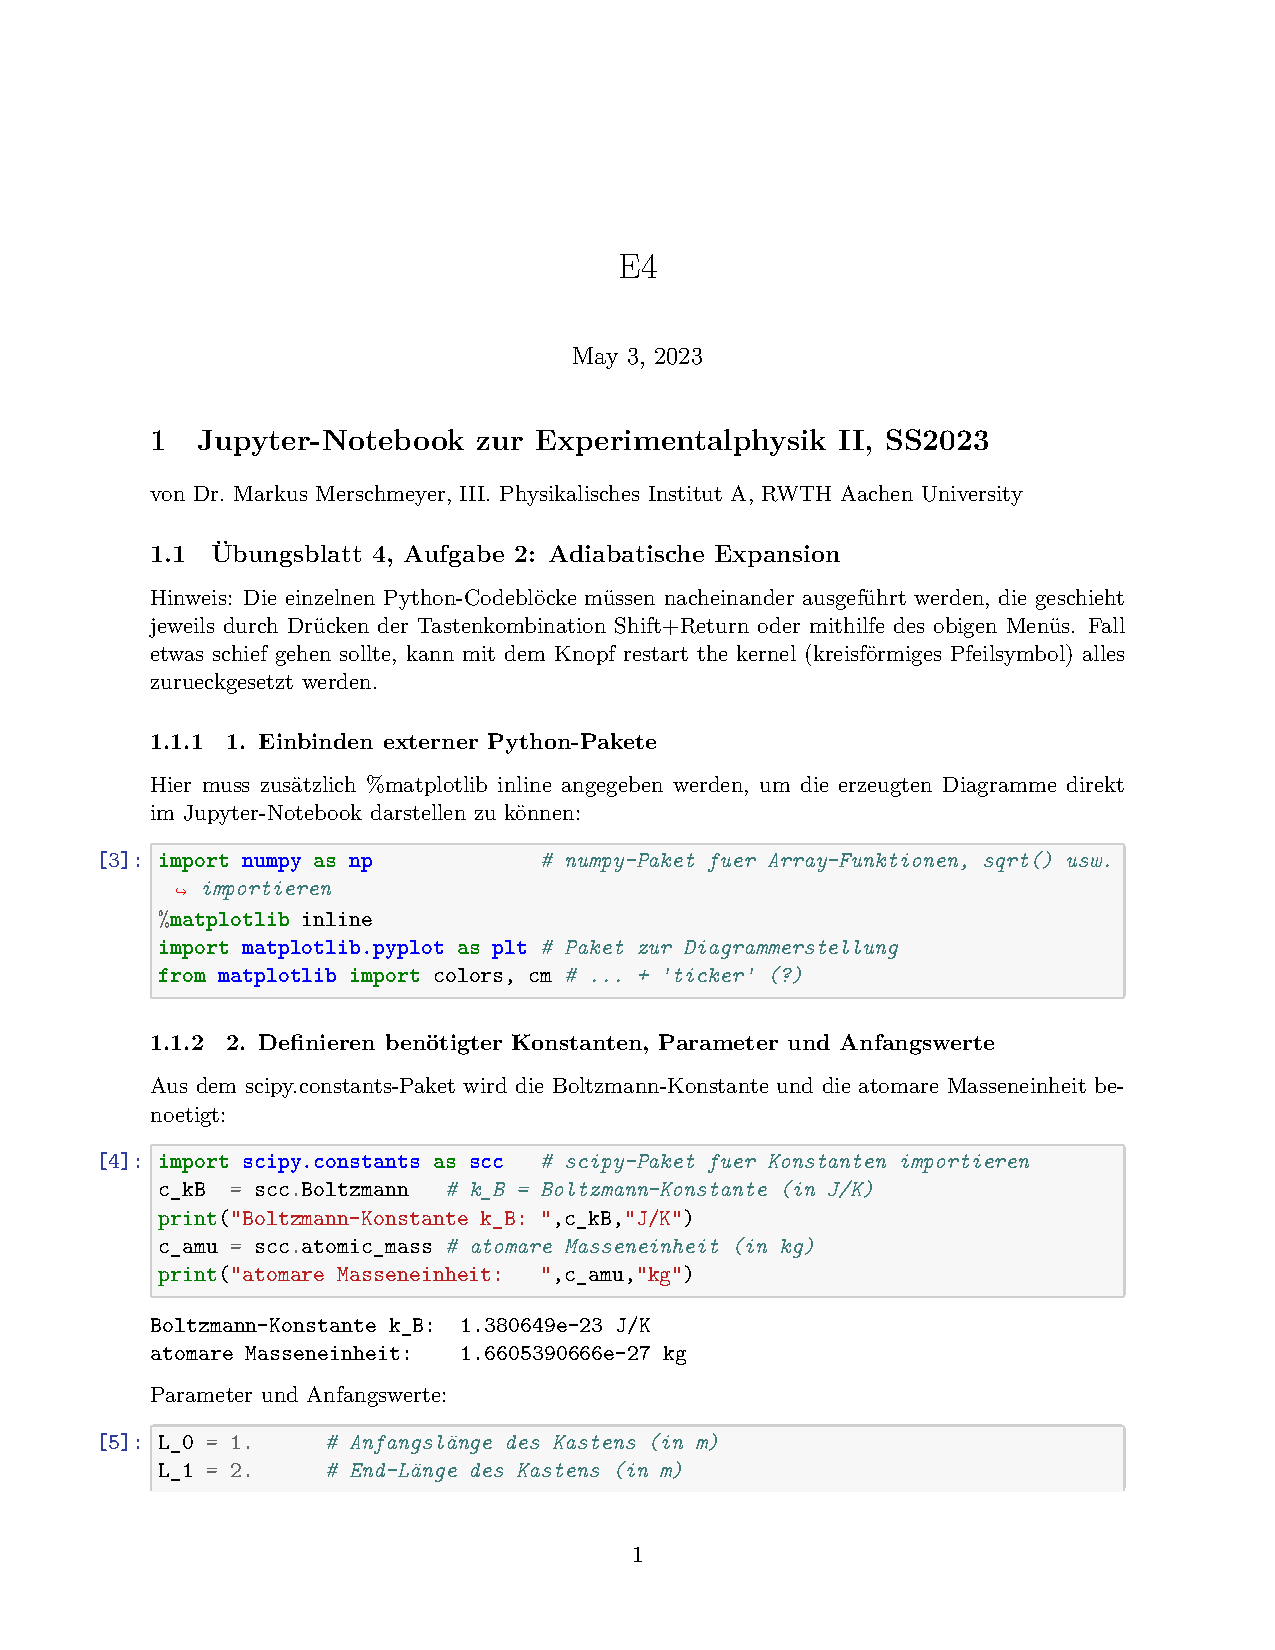
\includegraphics{E4_ipynb.pdf}

            \item
            \begin{align*}
                TV^{\kappa-1} &= \text{const}\\
                T'(2V)^{2} &= \text{const}\\
                4T'V^{2} &= \text{const}\\
                \frac{T'}{T} &= \frac{1}{4}\\
                \\
                \frac{\frac{p' V'}{N' k_B}}{\frac{p V}{N k_B}} &= \frac{1}{4}\\
                \frac{p'}{p} &= \frac{1}{4} \frac{V}{V'}\\
                \frac{p'}{p} &= \frac{1}{8}\\
            \end{align*}
            Die numerischen Ergebnisse stimmen fast exakt mit den analytischen überein.

        \end{enumerate}
    
    \item \textbf{Entropie beim Kartenmischen}
        \begin{enumerate}
            \item 
            \begin{align*}
                \Delta S &= k_B \cbrace{\ln n_{RM}'- \ln n_{RM}}\\
                &= k_B \cbrace{\ln N!- \ln 1}\\ 
                &= \cb \cbrace{\ln 52!- \ln 1}\\ 
                &\approx 2.16\cdot 10^{-21} \ufrac{J}{K} 
            \end{align*}

            \item 
            Aus einer statistischen Sicht, lässt sich der in (a) erhaltene Wert, als ein
            Maß dafür interpretieren, wie viele zusätzliche Informationen man über das System
            braucht, um den gegebenen Mikrozustand vollständig zu beschreiben. Der zweite Makrozustand
            (ungemischt) gibt somit weniger Informationen über den Mikrozustand als der erste 
            Makrozustand (geordnet).

        \end{enumerate}
    \newpage
    \item \textbf{Entropie und Reversibilität}
        \begin{enumerate}
            \item
            Da der Prozess irreversibel ist, gibt es erst mal keinen Umkehrprozess. 
            Hätte man die beiden Körper aber mittels
            z.B. einer Carnot-Maschine ins thermisches Äquilibrium gebracht, so hätte 
            man die gespeicherte Energie dazu benutzen
            können, um das System wieder aus dem Äquilibrium zu bringen. Alternativ
            ermöglicht dies auch externe Energie, mit der man den einen Körper kühlt, und den 
            anderen erhitzt.

            \item
            Sobald das System in das Äquilibrium übergegangen ist, wird es diesen
            nach dem zweiten Haubtsatz der Thermodynamik nicht mehr von alleine verlassen.
            Da bei dem Prozess auch keine thermische Energie in andere Energieformen umgewandelt
            wurde ist es somit nicht möglich, ohne weitere externe Energie, den Ablauf umzukehren; 
            Es handelt sich um einen irreversiblen Prozess.


        \end{enumerate}
    
    \item \textbf{Entropie: Kupferblock}
        \begin{enumerate}
            \item 
            Der Prozess ist äquivalent zu dem in Nr.4 und somit irreversibel. Um trotzdem 
            eine Entropie- differenz anzugeben, muss daher ein reversibler Äquivalenzprozess
            herangezogen werden. 

            \item
            \begin{align*}
                c_{\ch{H2O}} &= 4.2 \cdot 10^{3}\,\ufrac{J}{kg\,K} &
                c_{\ch{Cu}} &= 3.83\cdot 10^{2}\,\ufrac{J}{kg\,K}\\
            \end{align*}
            \begin{align*}
                c_{\ch{H2O}} m_1 T_0(\ch{H2O}) + c_{\ch{Cu}} m_2 T_0{\ch{Cu}} &= T_1 \cbrace{c_{\ch{H2O}} m_1  + c_{\ch{Cu}} m_2}  \\
                T_1 &= \frac{c_{\ch{H2O}} m_1 T_0(\ch{H2O}) + c_{\ch{Cu}} m_2 T_0(\ch{Cu})}{c_{\ch{H2O}} m_1  + c_{\ch{Cu}} m_2}\\
                &\approx 279\,\mathrm{K}\\
                \\
                \Delta S &= \int_{K} \frac{\di Q_{rev}}{T} \\
                &= \int_{K} \frac{\di U}{T}\\
                &= m c_{v}\int_{T_0}^{T_1} \frac{\di T}{T}\\
                &= m c_{v}\ln \cbrace{\frac{T_1}{T_0}} \\
                \\
                \Delta S_{\ch{Cu}} &= m c_{v}\ln \cbrace{\frac{T_1}{T_0}} \\
                &\approx 1\,\mathrm{kg} \cdot 3.83\cdot 10^{2}\,\ufrac{J}{kg\,K} \ln \cbrace{\frac{279\,\mathrm{K}}{373.15\, \mathrm{K}}}\\
                &\approx -112 \, \ufrac{J}{K} \\
            \end{align*}
            
            \item
            \begin{align*}
                \Delta S_{\ch{H2O}} &= m c_{v}\ln \cbrace{\frac{T_1}{T_0}} \\
                &\approx 5\,\mathrm{kg} \cdot 4.2\cdot 10^{3}\,\ufrac{J}{kg\,K} \ln \cbrace{\frac{279\,\mathrm{K}}{277.15\, \mathrm{K}}}\\
                &\approx 130 \, \ufrac{J}{K} \\
            \end{align*}

            \item
            \begin{align*}
                \Delta S_{ges} &= \Delta S_{\ch{Cu}} + \Delta S_{\ch{H2O}}\\
                &\approx -112 \, \ufrac{J}{K} + 130 \, \ufrac{J}{K}\\
                &\approx 18.3\, \ufrac{J}{K} 
            \end{align*}

        \end{enumerate}
    
\end{enumerate}

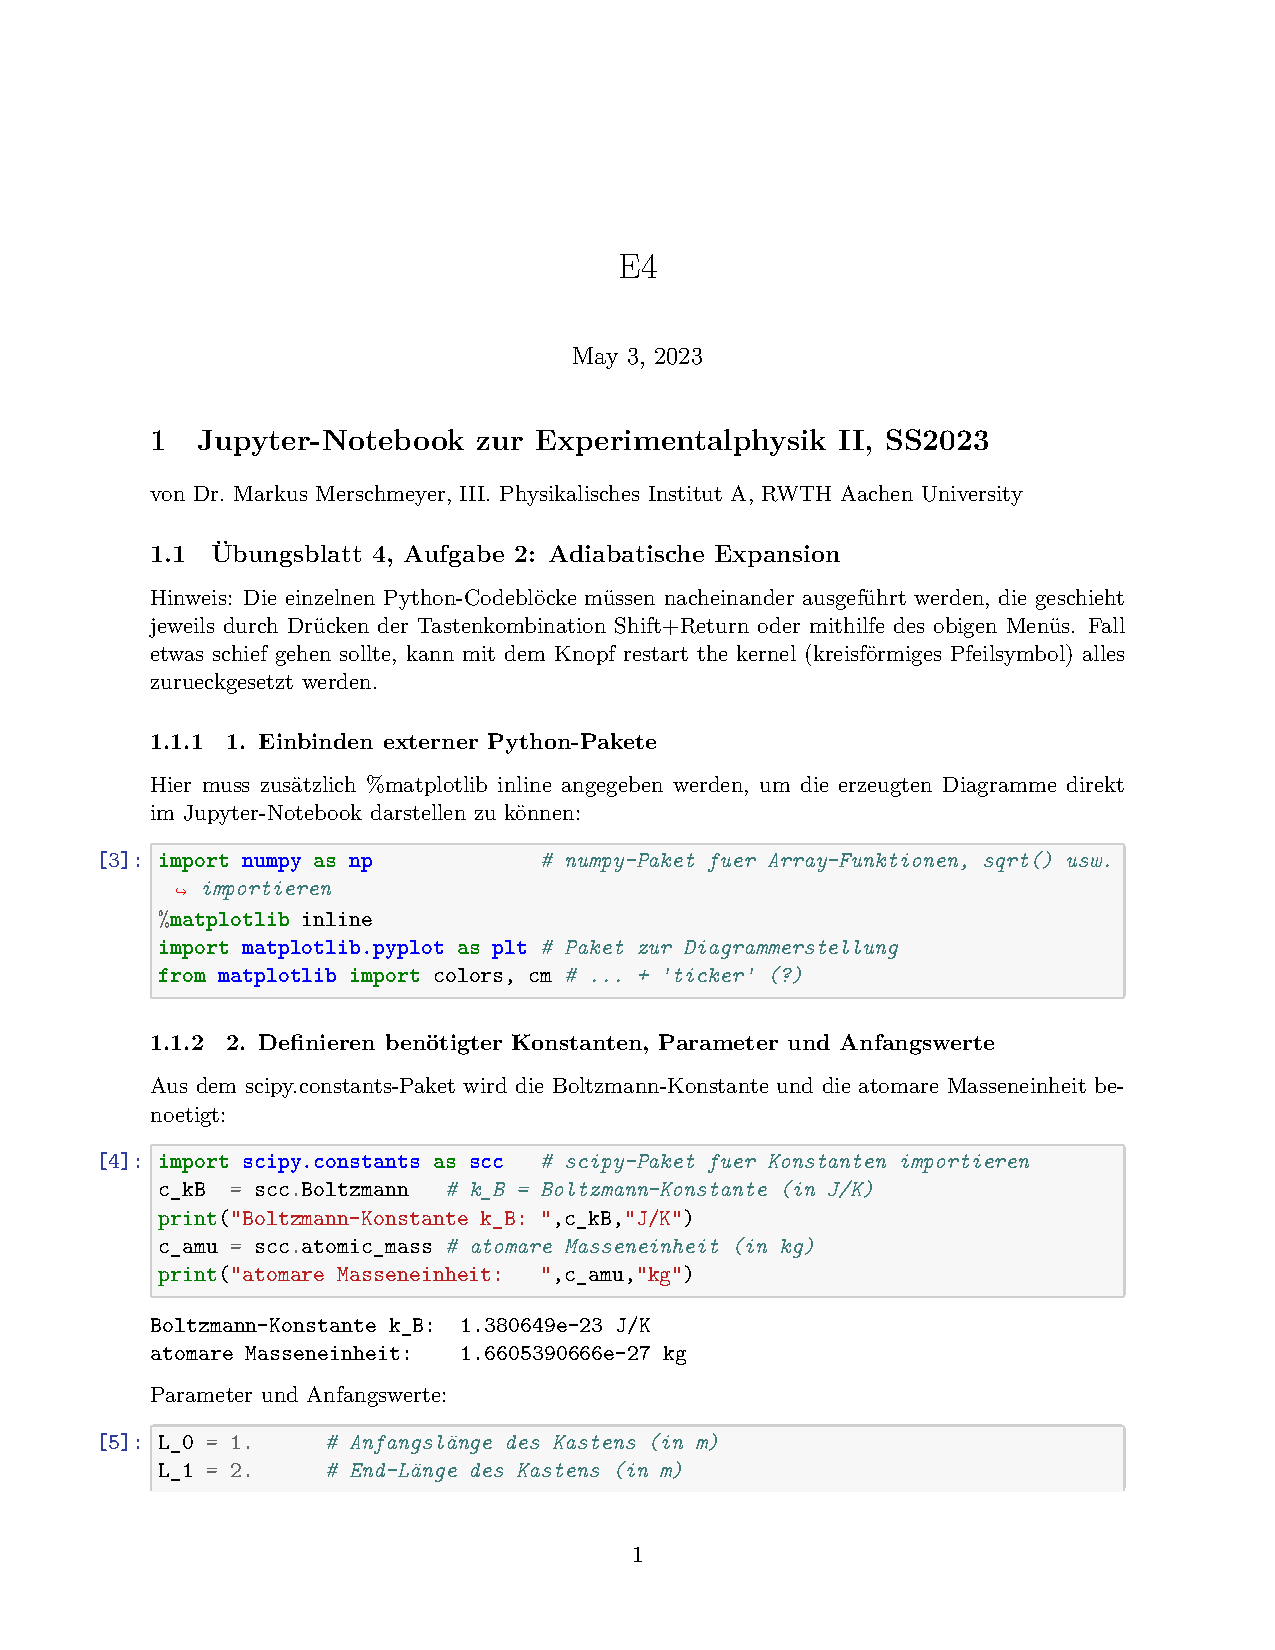
\includepdf[pages=-]{E4_ipynb.pdf}

\end{document}